\chapter{Convolution modelling of M/EEG data \label{Chap:data:meeg_artefact}}

\section{Overview}
	This chapter demonstrates an example of first-level modelling of M/EEG data\footnote{Supramodal EEG dataset: \url{https://www.fil.ion.ucl.ac.uk/spm/data/eeg_supramodal/}} using the convolution GLM introduced in \cite{Litvak_ConvModel_2013}. The example is based on a workshop held by B.\ Spitzer in 2015 (\href{https://github.com/bernspitz/convolution-models-MEEG}{see on GitHub}) and reproduces the results presented in \cite{spitzer2016rhythmic} for a single subject. 

	The experimental setup involved presenting visual, auditory, and somatosensory stimuli to subjects in a supramodal integration task. In this example, we aim to investigate the EEG response to different modalities of sensory stimuli, specifically visual, auditory, and tactile pulses. To compare the responses, we want to capture the average event-related response for each modality across trials. However, conventional methods of averaging across trials to generate an event-related potential are not suitable for this experiment because the delay between consecutive pulses can be as short as 100 ms, resulting in overlap of the responses over time. Therefore, we need to employ more elaborate techniques to disentangle -- more precisely, to deconvolve -- the responses over time.

	The convolution GLM provides a way to deconvolve the responses using a standard GLM with some particular regressors in its design matrix. In convolution GLM, the rows of the design matrix represent time, and the response regressors are obtained by convolving event indicators with a basis set. This allows us to model the possible overlap between responses to consecutive stimulis. Here, we will see how to parameterize the basis set and its duration, as well as the events, to perform convolution modelling in SPM. 


\section{The data}
	In the following, we will be analysing single subject data. Visual stimuli were white light-emitting diodes, auditory stimuli were 1 kHz sine tones, and somatosensory stimuli were square-wave electric median nerve stimulation. Subjects were presented with a standard sequence (N1) followed by a delay and then a comparison sequence (N2) which contained the same number of pulses as N1 ± 1 pulse. Subjects were instructed to respond by pressing a foot pedal after the N2 interval offset, to identify which of the two sequences contained the more pulses. EEG was recorded from 64 active electrodes and ocular activity was registered via two pairs of additional electrodes.

\section{Convolution GLM for M/EEG data}

	\subsection{Preparing the data}
		The data provided with this example have already been preprocessed. However, there are still a few preparation steps required: we need to re-reference, filter, and mark artifacts. To do so: 
		\begin{itemize}
		 	\item Start SPM in EEG mode. 
		 	\item Click on ``Prepare (batch)'' in the upper panel of the main SPM window, 
		 	\item Configure the ``Prepare'' batch: 
		 	\begin{itemize}
		 		\item Under file name, select ``dpil02.mat'', 
		 		\item Under ``Select task(s)'', select ``EEG referencing'' and leave defaults settings to reference against the average.  
		 	\end{itemize}
			 \begin{figure}[htb]
			 	\centering
			 	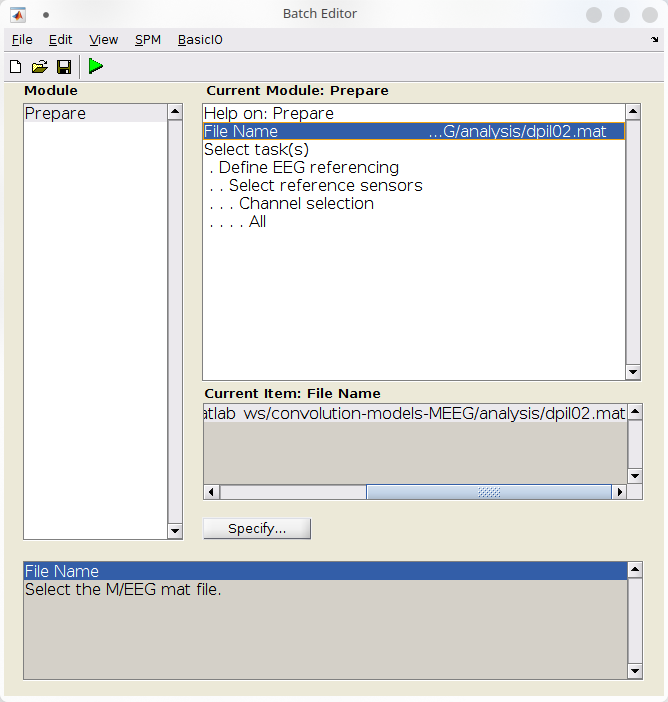
\includegraphics[width=0.6\textwidth]{meeg_firstlevel/figures/prepare-options.png}
			 	\caption{Options for the Prepare batch}
			 	\label{fig:meeg-firstlevel:prepare}
			 \end{figure}
		 	\item Add a ``filter'' batch (SPM \textgreater M/EEG \textgreater Preprocessing \textgreater Filter), 
		 	\item Configure a 5th-order Butterworth highpass filter at $0.5Hz$:
		 	\begin{itemize}
		 		\item Under file name, use the dependency button to refer to the file produced by the previous batch, 
		 		\item Under ``Band'', select ``Highpass'',	
		 		\item Under ``Cutoff(s)'', specify ``0.5'', 
		 	\end{itemize}
		 \begin{figure}[htb]
		 	\centering
		 	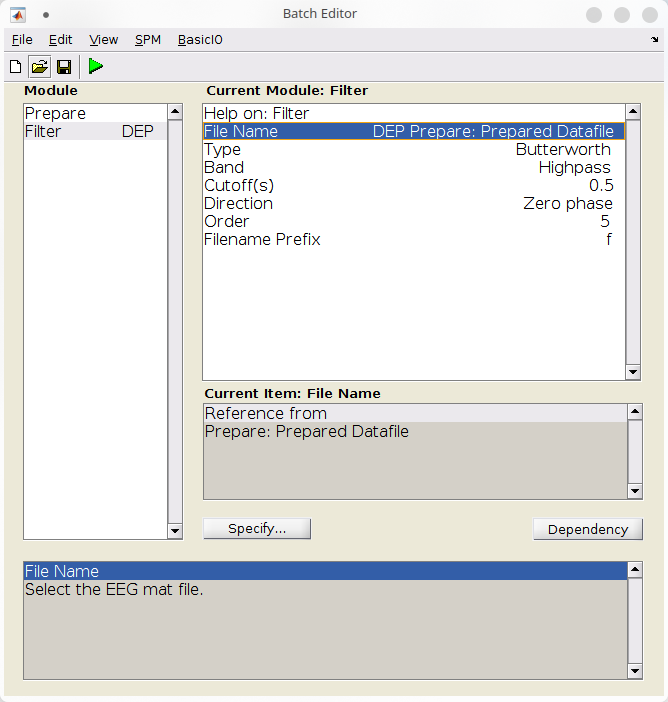
\includegraphics[width=0.6\textwidth]{meeg_firstlevel/figures/filter-options.png}
		 	\caption{Options for the Filter batch}
		 	\label{fig:meeg-firstlevel:filter}
		 \end{figure}
		 	\item Add an ``Artefact detection'' batch (SPM \textgreater M/EEG \textgreater Preprocessing \textgreater Artefact detection), 
		 	\item Configure the batch to mark artefactual samples: 
		 	\begin{itemize}
		 		\item Under file name, use the dependency button to refer to the file produced by the previous batch, 
		 		\item Under ``Mode'', select ``Mark'',	
		 		\item Under ``Detection algorithm'',  select ``Threshold channels'',
		 		\item Under ``Threshold'',  specify ``0.8'',
		 		\item Under ``Excision window'',  specify ``300'',
		 	\end{itemize}
			\begin{figure}[htb]
			 	\centering
			 	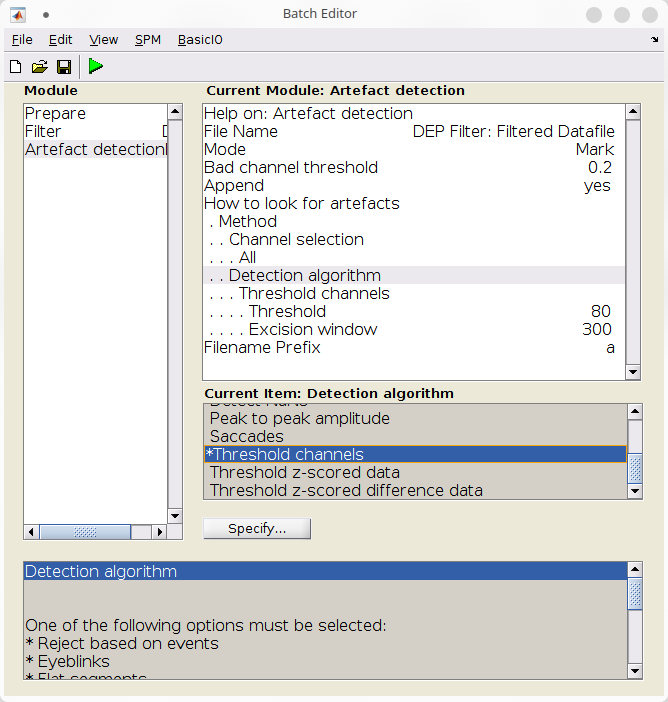
\includegraphics[width=0.6\textwidth]{meeg_firstlevel/figures/artefacts-options.png}
			 	\caption{Options for the Artefacts batch}w
			 	\label{fig:meeg-firstlevel:artefacts-options}
			 \end{figure}
		 	\item Run the batch with the ``Play'' button. 
		 \end{itemize} 
		 This batch should populate several files, the last being ``afMdpil02.mat'', containing the data that we will model with convolution GLM. 

	\clearpage

	\subsection{Constructing the convolution GLM model}
		\begin{itemize}
			\item Load the file called ``events.mat''. The events onset times are stored in 3 cells corresponding to visual, auditory, and tactile events.
			\item On the main SPM window, click on ``Specify 1st-level''
		\end{itemize} 
		Now we need to configure the batch for the convolution GLM analysis. 
		\begin{itemize}
			\item Specify the channels to model under ``Channel selection'':
			\begin{itemize}
				\item Remove the default entry (``Delete: All'')
				\item Click ``Select channel by type'' \textgreater ``EEG''
			\end{itemize}
			\item Specify the timing parameters
			\begin{itemize}
				\item Under ``Time window'', set $[-300 \;\; 700]$. This will model the response between 300ms before and 700ms after event onset. 
				\item Under ``Unit for design'', set ``seconds''
			\end{itemize}
			\begin{figure}[htb]
			 	\centering
			 	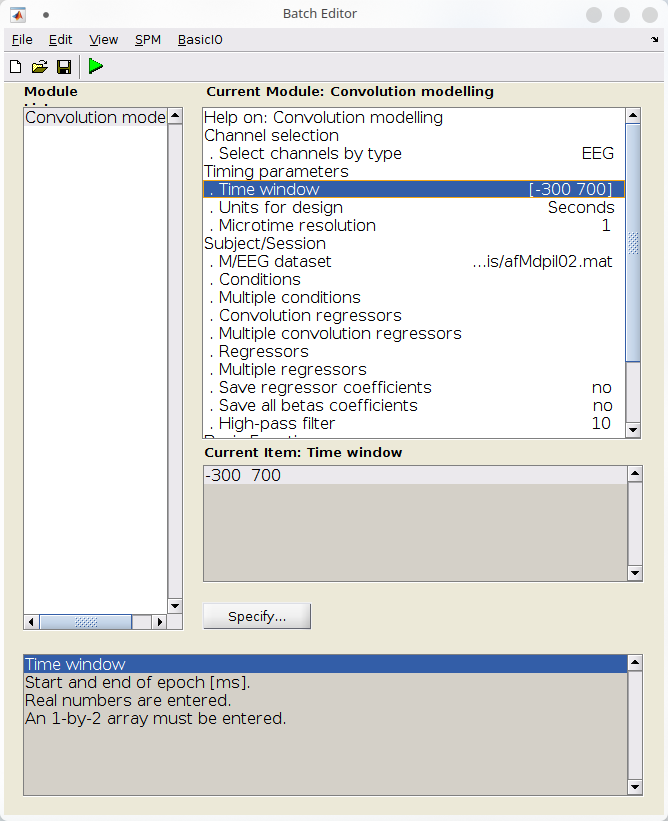
\includegraphics[width=0.6\textwidth]{meeg_firstlevel/figures/conv-top.png}
			 	\caption{Setting the channels and timing parameters of the convolution model}
			 	\label{fig:meeg-firstlevel:conv-top}
			 \end{figure}
			\item Specify the model structure
			\begin{itemize}
				\item Under ``M/EEG dataset'', select the last file produced at the previous section (``afMdpil02.mat''),
				\item We will now specify the events for each condition. To do so: 
				\begin{itemize}
					\item Click ``Conditions''\textgreater ``New: Condition'', 
					\item Under name, set ``visual'', 
					\item We will set the event times manually. Under ``How to define events'', select ``Manually''
					\item Under ``Onset'', type ``events\{1\}''. This corresponds to the event onsets times from the ``events.mat'' file for event 1
					\item Under ``Duration'', set 0. This will cause SPM to create stick functions at event onset. 
					\item Leave over parameters of that section to their defauls
				\end{itemize}
				\item Repeat the previous steps for  ``auditory'' and ``tactile'' events, whose onsets are stored in ``events\{2\}'' and ``events\{3\}''.
			\end{itemize}
			\begin{figure}[htb]
			 	\centering
			 	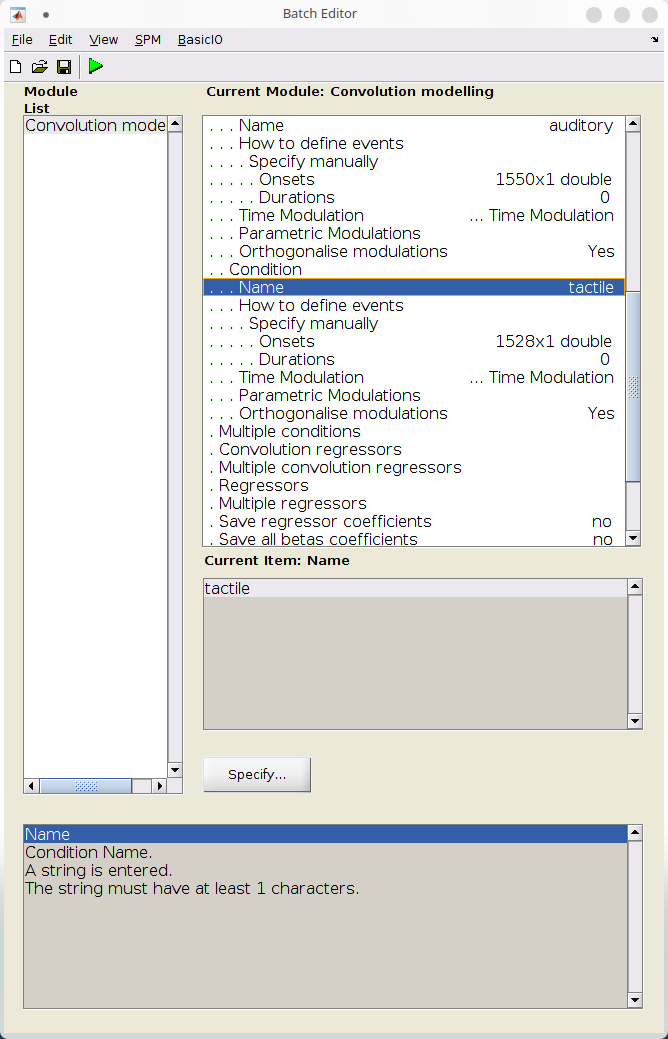
\includegraphics[width=0.6\textwidth]{meeg_firstlevel/figures/conv-other-conds.png}
			 	\caption{Specifying the conditions of the convolution model}
			 	\label{fig:meeg-firstlevel:artefacts-options}
			 \end{figure}
			\item The last important step is to specify the basis set and its order. Under ``Basis Functions'':
			\begin{itemize}
				\item Make sure that the selected basis set is ``Fourier Set''. 
				\item Make sure that the ``Order'' is 12. 
			\end{itemize}
			\begin{figure}[htb]
			 	\centering
			 	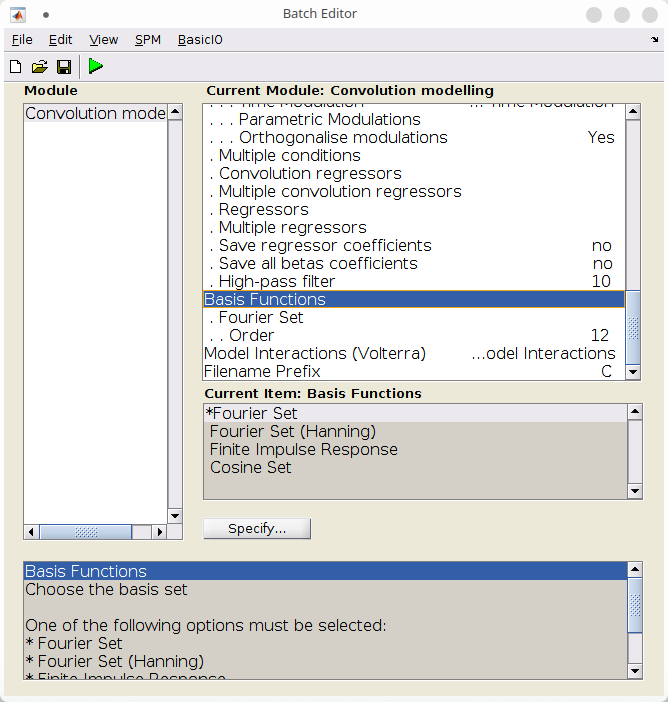
\includegraphics[width=0.6\textwidth]{meeg_firstlevel/figures/conv-basis-set.png}
			 	\caption{Setting the basis set of the convolution model}
			 	\label{fig:meeg-firstlevel:artefacts-options}
			 \end{figure}
		\end{itemize}
		A final step is to restablish the sensors type and locations using a Prepare batch (SPM>M/EEG>Preprocessing>Prepare). 
		\begin{itemize}
			\item Under ``File name'', click ``Dependency'' and select the output from the Convolution modelling batch, 
			\item Under ``Select task(s)'': 
			\begin{itemize}
				\item Click ``Set channel type'', and set ``New channel type'' to ``EEG''
				\item Click ``Project EEG sensors to 2D''
			\end{itemize}
			\begin{figure}[htb]
			 	\centering
			 	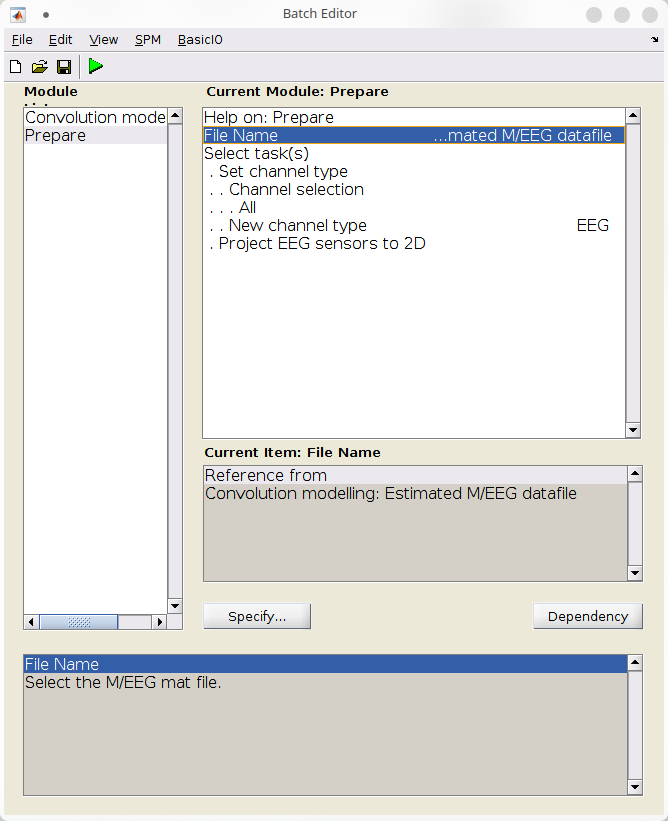
\includegraphics[width=0.6\textwidth]{meeg_firstlevel/figures/prepare-post-conv.png}
			 	\caption{Final prepare batch to fix sensors types and locations.}
			 	\label{fig:meeg-firstlevel:prepare-post-conv}
			 \end{figure}
		\end{itemize} 
		Finally, run the batch. 

	\subsection{Summary}
		To summarize, we have generated a Convolution GLM batch for our model to capture the response to each condition within a specific timeframe. Specifically, the design matrix created for this purpose has captured responses between 300ms before and 700ms after event onset, by expanding it on a 12th-order Fourier basis. This enables us to express the response as the weighted sum of 12 cosines and 12 sines, along with an intercept that captures the mean value. Note that the window of 1 second and the 12th-order Fourier basis allows us to capture oscillations between 1 and 12Hz, with a frequency resolution of 1Hz.

		Using SPM, the convolution GLM generates a new M/EEG dataset that contains the deconvolved responses as evoked data. Under the hood, SPM performs several operations: 
		\begin{itemize}
			\item First, it creates a design matrix $X$ for our problem $Y = X \beta + \varepsilon$, with time as rows and basis functions for each condition as columns.
			\item It then inverts the model to obtain an estimate of the parameters that weight the basis set, represented by $\beta = (X^TX)^{-1} X^T Y$. The rows of $\beta$ correspond to the weight of each basis function, stacked for each condition $c$.
			\item Lastly, it uses the basis function weights for condition $c$ to construct the deconvolved responses, represented by $y_c = x_{BF} \beta_c$.
		\end{itemize}

		Thus, the batch in this tutorial results in a M/EEG dataset of evoked responses, which contains three trials for each of our three conditions.

	\section{Results}
		The results can be visualized in the SPM's M/EEG viewer, which is in the ``Display...'' menu in the main SPM window. Selecting EEG and then clicking on the scalp image shows the deconvolved response over the scalp. By positioning the peristimulus time cursor tenth to hundreds of milliseconds after stimulus onset, we can observe the stereo-typical scalp maps of visual, auditory, and tactile stimuli (Figure~\ref{fig:meeg-firstlevel:scalp}). In summary, convolution modelling proves to be a powerful tool to disentangle responses that overlap over time (Figure~\ref{fig:meeg-firstlevel:responses}), and can be used as a preliminary step to extract event related responses for subsequent statistical analysis. 
		\begin{figure}[htb]
			\centering
			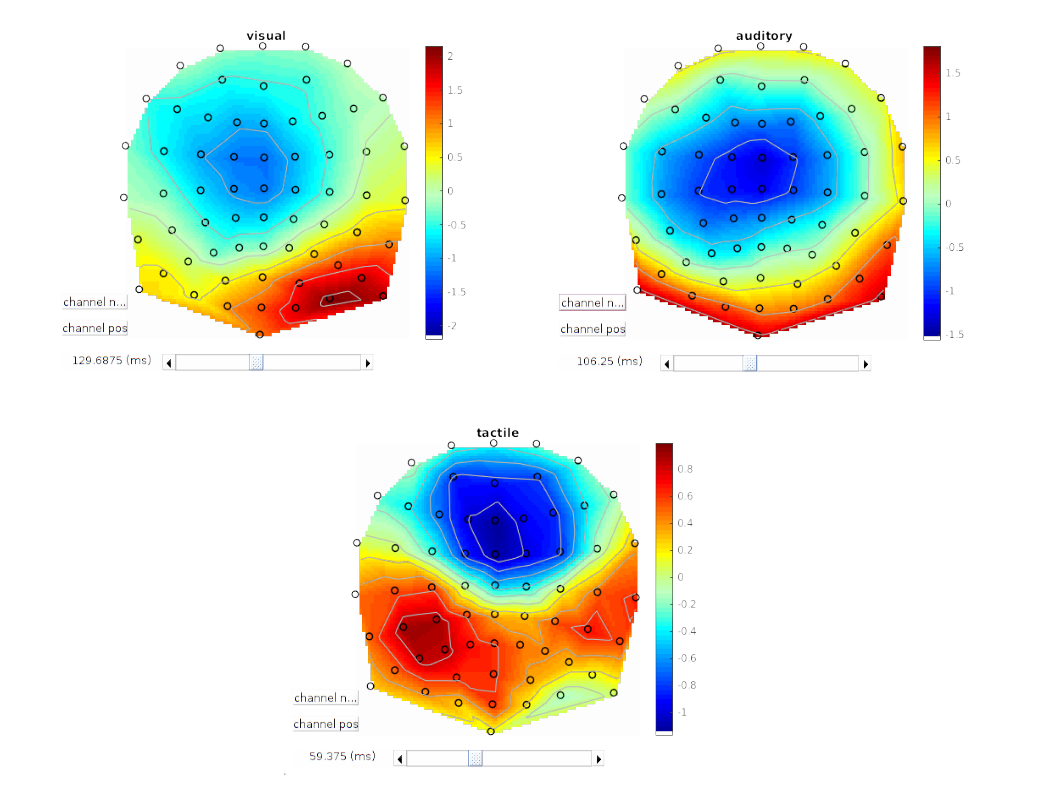
\includegraphics[width=0.9\textwidth]{meeg_firstlevel/figures/scalp.png}
			\caption{Scalp maps of deconvolved responses to the different stimuli at particular time of interest}
			\label{fig:meeg-firstlevel:scalp}
		\end{figure}
		\begin{figure}[htb]
			\centering
			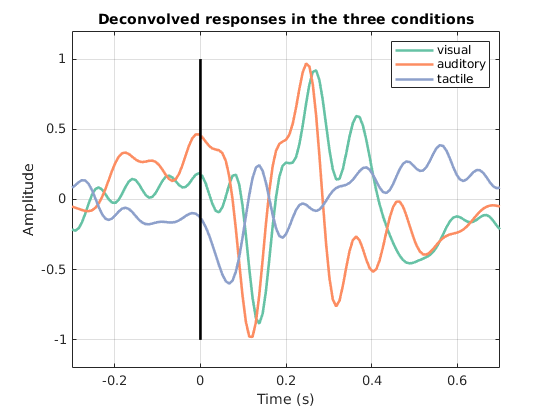
\includegraphics[width=0.7\textwidth]{meeg_firstlevel/figures/result-response.png}
			\caption{Average responses over fronto-central channels for the different stimuli}
			\label{fig:meeg-firstlevel:responses}
		\end{figure}

	\section{Acknowledgments}
		We thank Bernhard Spitzer for putting up the code from which this tutorial derives and for kindly allowing us to share the data analysed in this chapter.  